\documentclass[11pt, oneside]{article}   	% use "amsart" instead of "article" for AMSLaTeX format
\usepackage{geometry}                		% See geometry.pdf to learn the layout options. There are lots.
\geometry{a4paper}
\usepackage[parfill]{parskip}    			% Activate to begin paragraphs with an empty line rather than an indent
\usepackage{graphicx}
\usepackage{amsmath}
\usepackage{amssymb}
\graphicspath{ {images/} }
\usepackage{wrapfig}

% For adding the headers
\usepackage{fancyhdr}
\pagestyle{fancy}
\fancyhf{}
    \setlength{\headheight}{14pt}
    \lhead{150023118}
    \chead{CS3302 Practical 2}
    \rhead{November 24, 2017}
    \rfoot{\thepage}

\usepackage{fancyvrb}

\usepackage{tikz}
\usetikzlibrary{matrix,decorations.pathreplacing}

\title{CS3302 Practical 2: Hamming Codes}
\author{150023118}
\date{November 24, 2017}

\begin{document}
\maketitle
\section*{Overview}

The objective of this practical was to implement Hamming codes and allow the user to experiment with Hamming codes through a GUI. The user was to be able to specify a number from 2 to 6 for parameter \textit{r} and encode words with the corresponding Hamming encoding. Additionally, the application corrupts codewords at a certain probability, which the parity-checker tries to correct. The user is able to experiment with different error rates and parameters. 

\section*{Usage}

This application requires Python 3 (tested on version 3.6.3). Additional dependencies can be installed using

\begin{Verbatim}[tabsize=4]
	$ pip3 install -r requirements.txt
\end{Verbatim}

After all dependencies have been set up, the application can be launched with:

\begin{Verbatim}[tabsize=4]
	$ cd hamming_app/
	$ python3 flask_app.py
\end{Verbatim}

Once the application is running, the main window should be accessible on any browser at http://127.0.0.1:8080. 

\section*{Design}

This application was written as a Python web application that delivered though Flask. The code for the Hamming encoder and checker are included in \verb!hammingclasses.py!, which the user can interact with through the pages served by \verb!flask_app.py!

\subsection*{Hamming encoder and checker}

Instances of the class \verb|HammingEncoder| takes in a word and returns a codeword with the original bits in the word with parity bits attached. The constructor takes in the parameter \textit{r} as its argument and generates a Hamming encoder with a generator matrix.

The generator matrix is configured to place the parity-check bits at positions which are powers of 2. In other words, if $b_i$ stands for the bit at position $i$ (index $i-1$) and the set of all parity-bits is $P$, 

$$
P = \{\,b_i \mid \exists \, k \in \mathbb{N} \text{ such that } 2^k = i \ \& \ i < n \, \}
$$

Bit $b_i$ is an even parity-check bit on every data bit $b_j$ where $b_i \odot b_j \neq 0$; that is, 

$$
b_i = \bigoplus_{j}b_j \text{ for } \{\,b_j \mid b_i \odot b_j \neq 0\} 
$$

With this matrix, constructing codewords for each word becomes a matter of simply multiplying the word by the generator matrix. Since every number between 1 and n is uniquely represented in binary, it is also uniquely represented by a set of parity-check bits. Thus, this method allows us to construct generator matrix for Hamming codes of any parameter \textit{r} where any one corrupted bit would be identified.

The class \verb!HammingChecker! also takes in \textit{r} as the parameter, and constructs a checker matrix using the same algorithm. Codewords are checked by multiplication with the checker matrix. If the resulting vector matches up with any row in the checker matrix, the bit of that row has been corrupted. If the resulting vector is a zero vector, no corruption has taken place. 

\subsection*{User interface}

The user interface includes three components: a encoder page where the user can test the Hamming encoder and checker, a statistics page where the user can view statistics on the success rates of Hamming codes under various conditions, and a visualization page that shows related information as graphs.

\subsubsection*{Hamming encoding page}

When the application is launched, the user should be greeted with a page that looks as follows.

\begin{center}
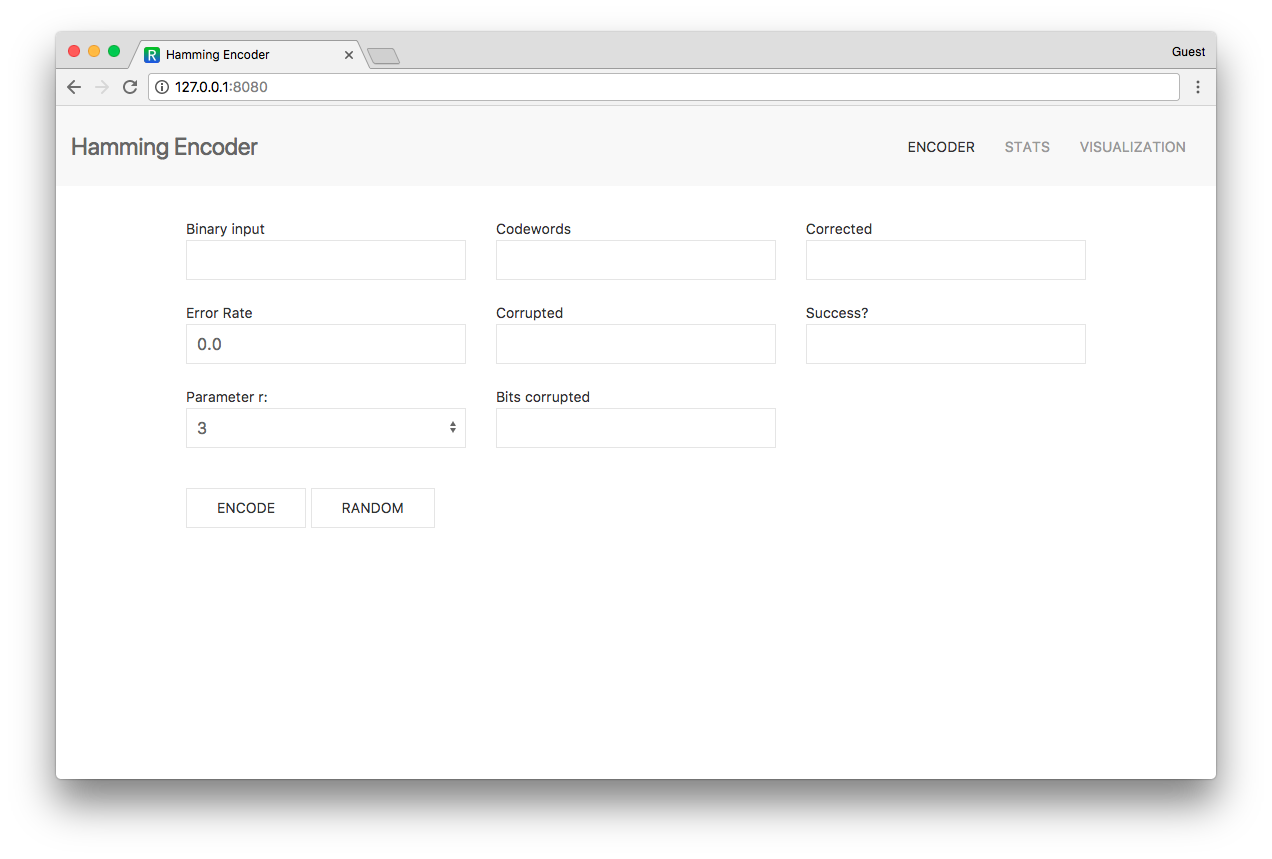
\includegraphics[width=345px]{main_blank}
\end{center}


The user should enter a word to encode, the error rate (the probability that any individual bit will be corrupted), and the parameter \textit{r}. When the encode button is pressed, the resulting codeword, the codeword after corruption, the number of bits corrupted, what the checker corrected the corrupted codeword to, and whether or not it matches up with the original codeword will be displayed. 

\begin{center}
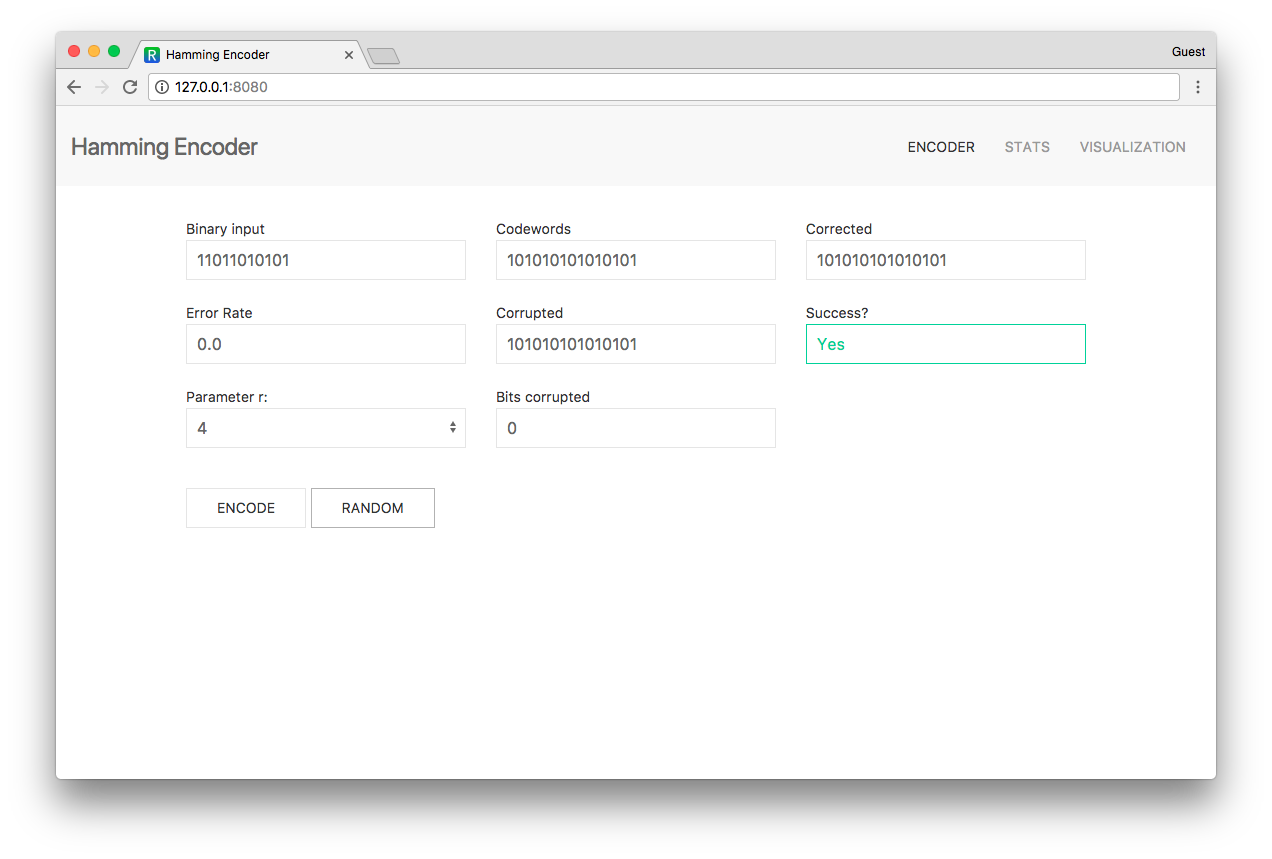
\includegraphics[width=345px]{main_code}
\end{center}

The user can then verify that any codeword that has one or fewer corrupted bits is corrected to the original codeword, whereas correction fails for any case where two or more bits are corrupted. Additionally, the random button generates a random word of length $k = 2^r - r - 1$. 

\subsubsection*{Statistics page}

The stats page allows the user to examine what the probability that the codeword will be successfully received at the other end after checks based on how reliable the transmission channel is. The user can specify what error rate is?that is, the probability that any individual bit will be corrupted?and the number of tests that they wish to conduct. The page will then display something like the following:

\begin{center}
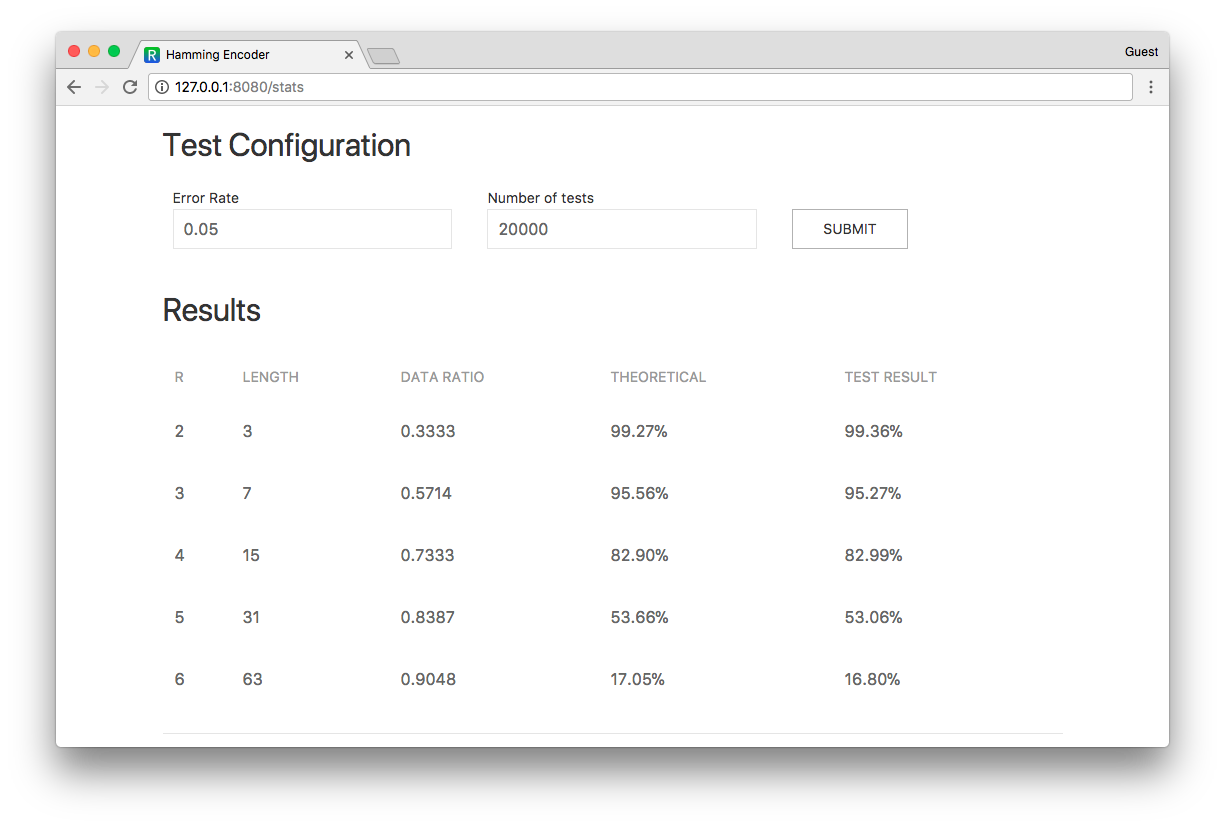
\includegraphics[width=345px]{stats2}
\end{center}

With this, the user can verify that the results of the tests approach the theoretical result as they increase the number of tests. The theoretical success rate is the probability that only 0 or 1 bits are corrupted, that is:

$$
p_{theory} = (1-p)^n + n \cdot p \cdot (1-p)^n
$$

After seeing how well Hamming codes of various sizes perform under a given error rate, and examining the ratio of data to total message length, the user can decide which parameter \textit{r} they wish to use for their use case. 

\subsubsection*{Visualization page}

The visualization page shows a line graph of the probability of a codeword being transmitted after Hamming checks given an error rate of p. Each of the lines corresponds to a different parameter for r. 

\begin{center}
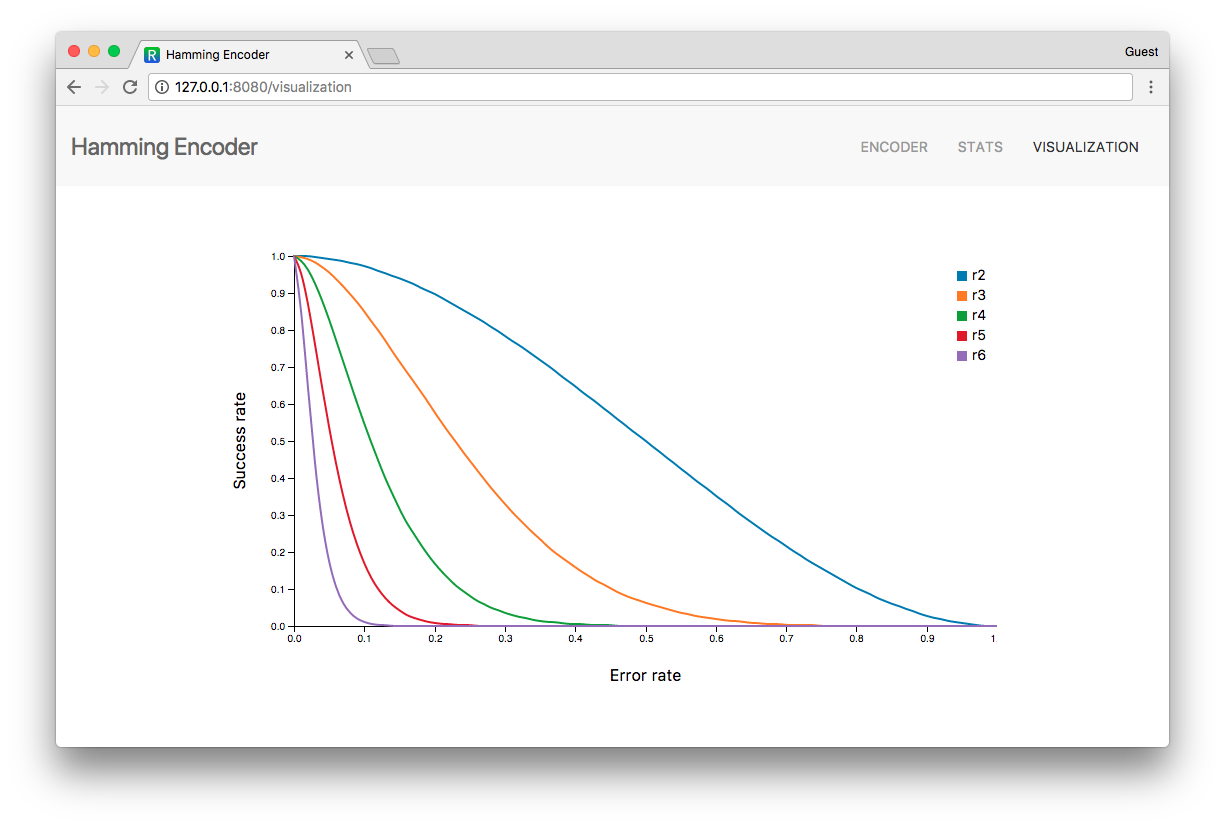
\includegraphics[width=345px]{vis1}
\end{center}

This visualization make it clear that although all variations of Hamming encoding transmit 100\% of their information at $p=0$ and converge to 0\% as $p$ approaches 1, the larger Hamming codes quickly become unworkable at fairly low $p$ values. 

\section*{Testing}

Unit tests have been included in \verb!basictests.py!. The tests check Hamming encoders and checkers with parameter \textit{r} set from 2 to 6. It verifies that the Hamming checker correctly identifies a codeword which has not been corrupted, successfully corrects a codeword when only one bit has been corrupted, and fails when two bits are corrupted. All 15 tests pass successfully. 

\section*{Analysis}


\begin{wrapfigure}{r}{6cm}
\vspace*{-1.3cm}
\centering
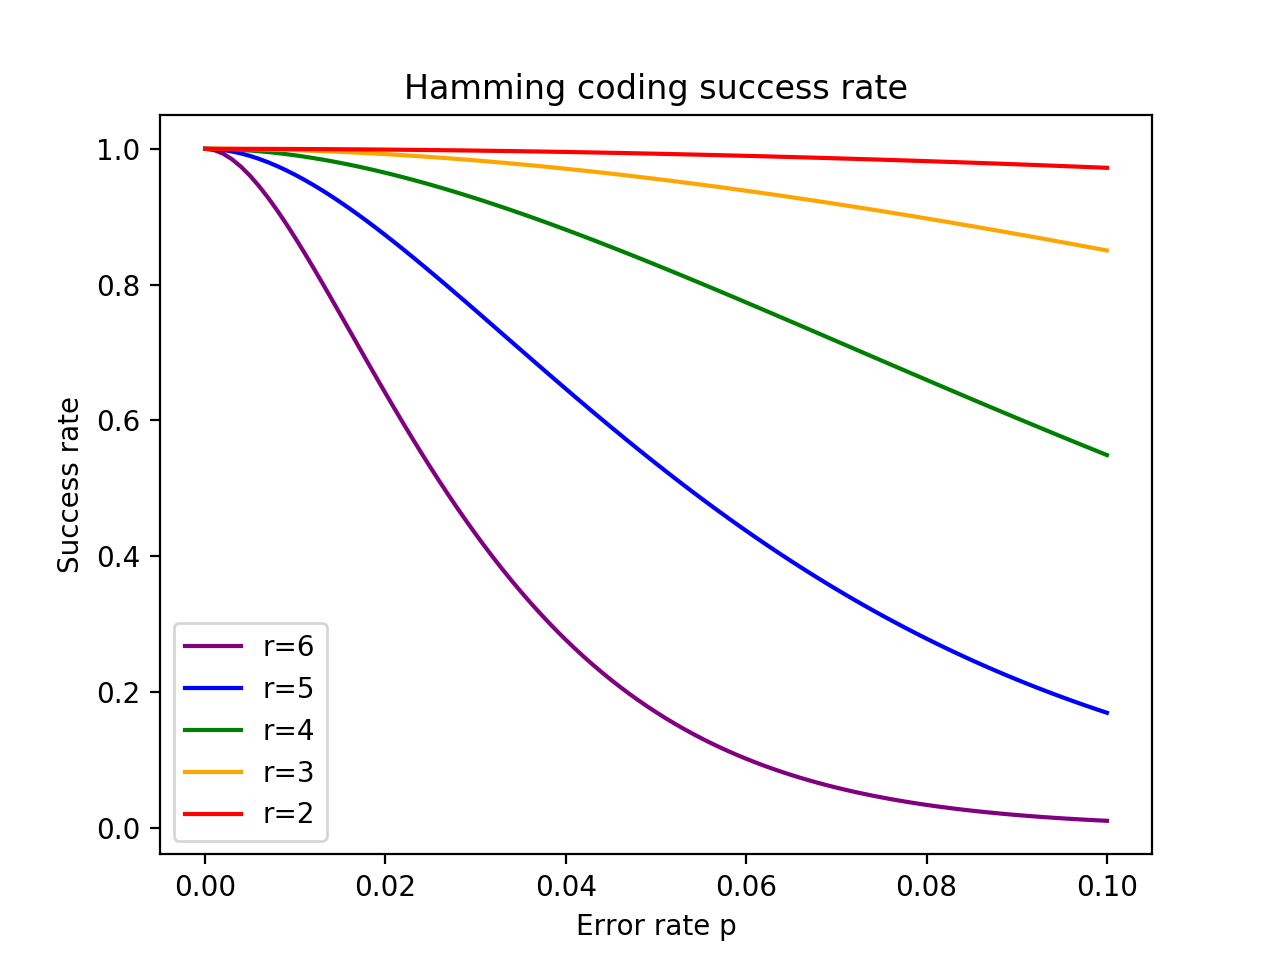
\includegraphics[width=0.48\textwidth]{figure2}
\end{wrapfigure}

As the reliability of Hamming codes can be calculated using the theoretical value, there is no need to test for each value of \textit{n} and \textit{r}. After analyzing the theoretical value, we can see that for example, in order for 99.99\% of codewords to be transmitted correctly, \textit{p} must be around 0.00578 or less with r=2, and 0.00219 or less with r=3.

Similar calculations can be made for any p. 
\end{document}  














